
\section{Introduction}
The digital electronic equipment’s evolution, in terms of local processing, low-cost and low power consumption, has been responsible to the growth of the distributed processing sensor nodes in the current networks. In special, in wireless networks, such as wireless sensor networks (WSN) or wireless mesh networks (WMN), the distributed processing can improve the network intelligence in terms of logistics and organization. With the rapid technological development of sensors, WSNs will become the key technology for Internet of things \cite{IEC2014}.

Sensor nodes are electronic devices, which typically contain sensors, a microcontroller, a radio communication chip and other peripherals. They can communicate with other nodes to form self-organization WSNs \cite{Son2009}. Wireless mesh networks (WMNs) are an emergency outdoor WLAN solution that can connect entire cities \cite{Akyildiz2009}.

Commonly, traditional networks rely on wired access points. In both WSNs and WMNs the connection between the nodes is implemented wirelessly. Mesh nodes or wireless sensors are typically wireless transmitters similar to wireless routers.

A WSN is a network formed by a large number of sensor nodes where each node is equipped with a sensor to detect physical phenomena such as light, heat, pressure, etc. \cite{IEC2014}. A WMN can be classified as a client, infrastructure or hybrid mesh network. In these cases, both mobile client devices and infrastructure nodes (mesh routers) provide routing and forwarding functionality \cite{Piezhao2008}.

Wireless mesh and sensor networks are spreading both in city and rural areas to connect heterogeneous home users. Their aim is to support (mobile) users seamlessly with cheap and easy to maintain connectivity \cite{Matos2013, Bhagwat2003, Johnson2007}. Considering their main application, the typical hardware constitution and the environment where they are normally implemented, the context-aware routing could improve the performance of the network.

The main requirements to the WSN's design are the low power, the scalability of the network, small size and the flexibility to be adapt to demanding applications \cite{Leon2015}. Being aware of such requirements, has been investigated the use of a link state routing protocol, the wireless extension Open Shortest Path First (OSPF), which is the current Internet standard for interior routing, has been extensively studied \cite{Holter2010, Fuertes2012}.

OSPF is the standard interior routing protocol widely deployed in the wired Internet (fixed nodes). Wireless OSPF is targeted at extending OSPF in a mobile ad hoc environment in which reducing protocol overhead is of paramount importance \cite{Holter2010}.

Generally, traditional wireless networks are based on routing protocols to find the best route to the gateway to reach the Internet without a contextualized concern, or without the knowledge of the environment in which it is allocated. In context-aware routing the environment gleaned information is used to adapt the network behavior to change its routing process.

Context information can be understood like a set of environment parameters that can be used to build optimized networks routes considering the environment information. The environmental awareness networks are able to connect the users, following the optimization use of the resources, modeled by the context information.

In this paper, the context-aware networks are investigated, considering the luminosity, temperature and humidity environment influence. The environment context is considered in the network best route solution.


\begin{figure*}[!t]
	\centering
	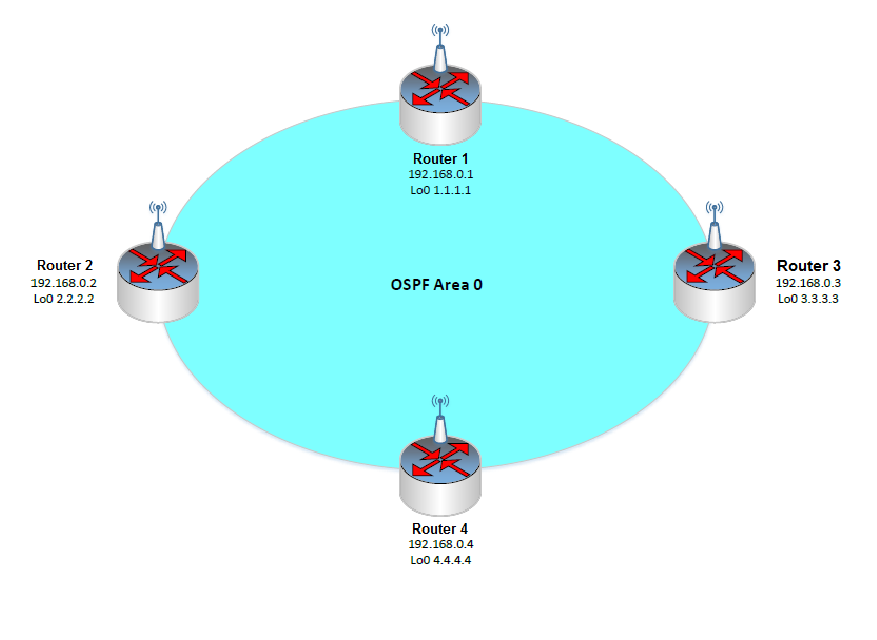
\includegraphics[width=0.7\textwidth]{figs/topology.eps}
	\caption{Wireless Network topology.}
	\label{Fig01}
\end{figure*}

The remainder of this paper is organized to present the components and the architecture of a wireless network based on context-aware routing. In Section II, the traditional routing protocols are revisited. In Section III, the environment parameters that may modify the routing context are presented. Section IV describes the results on the context-aware routing implementation for a wireless mesh network. Finally, in Section V, conclusions remarks are drawn.